\documentclass[12pt]{article}
\usepackage{amsmath}
\usepackage{enumitem}
\usepackage{float}
\usepackage{wrapfig}
\usepackage{graphicx}
\usepackage{caption}
\usepackage{titling}
\usepackage{enumitem}
\usepackage{parskip}
\usepackage{pgf}
\usepackage{tikzit}
\usepackage{pdfpages}
\usepackage{booktabs} % For formal tables

\input{tikz.tikzstyles}
\linespread{1.1}
\usepackage[hidelinks]{hyperref}
\hyphenpenalty=100
\newcommand{\ts}{\textsuperscript}
\usepackage[a4paper, portrait, margin=2.54cm]{geometry}
\title{{
\includegraphics[width=0.5\textwidth]{figures/ensae.png}\\
Applied stats project:\\ Technological proximity and innovation strategies\\}}
\author{Claire BRESSON, Thomas CHEN,\\ Elvis GABA-KPAYEDO, Patryk WISNIEWSKI\\[0.25cm]
Cycle Ingénieur 2A, ENSAE \\[0.25cm]
Supervisors: Antonin BERGEAUD, Clément Malgouyres}
\date{May 16, 2024}
\begin{document}
\begin{titlingpage}
\maketitle
\begin{abstract}
Innovation significantly improves both social and private firms' welfare. Patents grant inventors exclusive rights, encouraging innovation by providing temporary monopolies and facilitating knowledge dissemination. However, strategic patent use, such as blocking patents, can both inhibit and stimulate innovation. Using patent data from the Google Patents Database, we map firm-level innovation networks and analyse the impact of strategic patenting on these networks. We employ a microeconomic model and a difference-in-differences and network approaches to investigate effects of firm blocking behaviors on innovation levels and patent value.
\end{abstract}
\end{titlingpage}
\tableofcontents
\clearpage
\section{Introduction}
Innovation as the result of technological and scientific progress plays a key role in global social welfare through a change in working conditions or production of goods that improve daily life. As scientific progress, innovation is heavily dependent on a favourable environment consisting of different actors, research investment strategies as well as conducive policies whose interactions and behaviour dictate the pace at which innovation grows and determine its social and private returns. In order to empower innovation, public policies are shaped to foster knowledge exchange, as many empirical studies show that innovation is a cumulative process for new findings arise on the basis of past work. On the other hand, they aim at ensuring satisfying private returns for innovative actors, rewarding inventive activities, regarding the substantial amount of money involved (essentially by firms) in R\&D activities. Patents are the most common used instruments for protecting intellectual property and are defined as "government-issued rights granting inventors exclusive control over their inventions for a limited period". Indeed, patents are granted to inventors who have participated in the global innovation process through their research and offers a temporary monopoly to incumbent firm, which enables it to charge above its marginal cost and extracts innovation rent. In return for making its invention public, thus actively participating in the knowledge exchange, the firms receive a competitive advantage on its opponent. The latter consideration gives rise to new reasons for patenting (Corbel, 2004) and tends to move patents away from their traditional uses. To maintain this dominant position as long as possible, a firm may have to rely on various patenting strategies whether to prevent opponents from building on its current work to develop better products or actively hinder the efficient use of another firm's own invention eventually forcing them to enter cross-licensing negotiation, through the production of “blocking patents”. This behaviour has ambivalent effects ; On one hand, it can have inhibitive effects overall innovation. On the other hand, one can argue that it can stimulate it by forcing firms to be creative and develop their own directive line. The aim of this paper is to use patent data to infer the impact of these strategies. Using Google Patents Database, we use forward citation patterns and patent closeness measure from Google Patent  to map a firm’s network. This approach used in (Acemoglu, 2016) shows that “an innovation network acts as a conduit to the cumulative process of technological and scientific progress” after building a sector-level network. This motivates our construction of a firm’s network to further analyse the impact of patent’s strategic use of patents by a focal firm on the overall innovation inside the sub-network it belongs. Given the difficulty to identify ad-hoc strategies using patent data, we build a microeconomic toy-model to describe the reaction of representative firm to the grant of a patent given the centrality of the incumbent firm to further investigate the effects on patenting level in sub-network as well as the effect on patent real value measure as defined in ( Kelly et al, 2020) and use DiD to test our hypothesis. This paper is organised as follows.  It is crucial to understand the complexity of the notion of patents, which will be at the founding of the analysis: hence a review of the previous literature on the subject. This review will tackle the concepts of patent value, of innovation network  in order to grasp the interactions between firms' strategies. Then a focus on the data that has been used and its visualisation through descriptive statistics will give better insight into the material and what can be understood thanks to it. After that, the methodology and the models implemented will be explained, in order to make it clear how the results were obtained. The next section will consist in the presentation of these results. Eventually, the conclusion of the paper will summarise how this research contributes to a global reflection around patents and innovation and open further perspectives. 

\section{Literature review}
\subsection{Definition and benefit for the inventor}
Patenting has been developed in order to entice people to innovate (because innovation is seen as something positive that will benefit the society as a whole). Indeed, because innovation is often costly, it may appear as a public good: its benefits are public but its costs are private. All the agents in the market want it developed but none wants to undertake the developing costs. As a consequence, there might be no innovation at all. Thus, patenting systems were imagined as a means to implement a reward for innovation: an inventor who patents his invention will be granted, for a certain period of time, a monopoly. A monopoly is highly desirable for a seller because it yields him a greater profit than a competitive market would. Thus, even if the implementation of patents may seem detrimental to consumers in the short run, they are considered as a necessary evil to ensure a global improvement of things in the end. 

As explained above, patents are part of companies' strategies in order to maximize their profit. There are two main motives for getting a patent, which enable one to classify patents into two categories (even if the frontier is sometimes blurred). The first motive, the most evident of the two, corresponds to an “offensive patent strategy”: firms try to get patents that will open new markets for them and in that case, they innovate. The second motive for getting a patent is a “defensive” one: patents prevent competitors from imitating the innovating inventions of the firm, which may even impede them to further develop the patented invention. So the patenting system, though certainly favouring innovation in many cases, can also be an obstacle to it. The motivation of a patent is highly correlated to its content: an offensive patent is by definition far more innovative than a defensive one. 

Such are the motives of companies to get patents. Now let us focus on patents themselves.

\subsection{Computing a patent's value}
A difficult question to tackle about patents is the computation of a patent’s value. How should patent value be defined? There are two main concepts that must not be mixed up: the private value of a patent, which is how much it benefits its inventor, and the public value of a patent, which is how much it benefits society as a whole, essentially measuring its level of innovation.

For some time, because patents can be a way of measuring innovation and because innovation is a driver of growth, economists have mainly focused on the public value of a patent. To compute the public value of a patent, researchers study the number of citations a patent receives in subsequent literature. If a patent is cited frequently, it suggests it has been a breakthrough in innovation, influencing many subsequent research papers. Conversely, a patent that is never cited in the following years is likely not a significant innovation.

One must think carefully before choosing the period over which to look for citations of a given patent. Should all subsequent patents be observed, or only those in the nn years following the issuance of a patent? Depending on the choices made, the results might differ, and the patents identified as the most innovative will not be the same.

\textbf{Measuring private patent value}

However, to fully understand patent strategies, one must also focus on the private value of a patent. This is the aim of Technological innovation, resource allocation and growth, Kogan et al. The authors designed a metric to measure the private value of a patent. It may differ from the scientific value: for instance, a patent that is very successful in restricting competition, even if it is not a breakthrough innovation, will have a high private value (and low scientific value). The metric is based on the fluctuations in the company’s stock price. Indeed, it is reasonable to think that if a patent is valuable for the company, it will have an impact on its stock price. The first step of the analysis is to identify the release of information on the market. The market first learns about the application for the patent, which influences the stock price even before the patent is issued. Then, when the issuance is effective, the market learns that too. Here it is considered that within 3 days after the issuance of the pattern, this new piece of information will be reflected on the firm’s stock price. After that comes the question of isolating the effect of the patent issuance from all the other factors which may impact the company's stock price. Market movements may be controlled by focusing on the firm idiosyncratic return (firm return minus market portfolio return). One limit to the model is that it supposes that the market knows the patent value from the time of the application (as opposed to the time of patent issuance): that became true after some 2000 regulation but was probably not true before, which may lead to overestimating the market reaction. Yet, the checkings conducted by the authors show that the consequences of that assumption are not really significant. 

Interestingly, though this model measures private value whereas citations-based models measure scientific value, the article notes that both are significantly linked.

Then comes the question of the link between this measure and firm growth. First, the authors define firm innovation as the sum of all patent values, weighted by the number of future citations. After that, they study the relation between, on the one hand, a given firm's innovation and that of its competitors and, on the other hand, the firm's future growth and productivity. They control the analysis by size, firm idiosyncratic volatility, industry and time. Overall, they prove that their measure is related to productivity and growth. They show that their measure captures more information about the quality of patents than citations-based measures do and that it enables them to evidence patterns of creative destruction. Aggregating innovation coefficients, they find that at the aggregate level, innovation is linked with resource reallocation and growth. When using aggregate innovation index, it turns out that waves of innovation trigger an acceleration of output and productivity growth.

Thus, this study shows that one must bear in mind the difference between a patent’s private value and its innovative level; it also demonstrates that these two figures can be computed through distinct methods. 

\subsection{Measuring patent significance}
In “Measuring technological innovation over the long run”, Kelly et al. study patent “significance”, that is to say the innovative value of a patent. They do it through text analysis on patents issued between 1840 and 2010. The aim is to evaluate the change brought about by the invention patented and its impact on future research and development. To do so, the economists compare the text of the patent studied with that of posterior patents, in order to measure the similarities in the vocabulary used. First, they develop a metric to measure these similarities, which identifies specific words (words that are not cited in many documents, contrary to common words) and gives them higher weight in the calculation. Then they compute patent's "backward similarity", which is to say its similarity with the existing stock of patents (patents that were developed in the $n$ years before the issuance of the studied patent) and its "forward similarity" (similarity with patents issued in the $n$ years following the issuance of the studied patent). The ratio of the two gives the value of the studied patent's significance because it takes into account both the novelty of the patent (similar or not to prior ones) and its impact on future research and development (similar or not to subsequent patents). A very significant patent would then be one whose content is very different from what existed before and very similar to what was developed after. Both the indicators ars important because a patent with high "forward similarity" but also high "backward similarity" is one that is part of an innovation process but without being a turning point in this process. On the other hand, a patent with low "backward similarity" but also low "forward similarity" has no impact on further development, which means that it cannot be a paramount innovation. 

The authors check the validity of their measure with historical patents and by comparing their results to those obtained with the forward-citation method (method mostly used when one tries to evaluate the innovative level of a patent). The model seems consistent and more precise. It is thus an interesting measure when one tries to understand where the value of a patent comes from. 

Moreover, the article raises the question of the link between patent significance and patent market value. As explained above, patents may have different public and private value and it might be difficult to know exactly where market value stems from. Kelly et al. thus compare their measure of patent significance with the measure developed by Kogan et al., which describes patent private value. They find that there is a significant relation between the two.

The authors also explain how their measure can be used to measure innovation over the long run. They define breakthrough innovation as the top 10\% more significant and design a time series with the number of breakthrough innovations per year and per American. That gives an overview of innovation and its fluctuations over a rather short period of time. 

Finally, one can focus on the relationship between patent significance and productivity (using productivity indexes developed by economists earlier on). Both at the aggregate and at the sector levels, the analysis shows that there is no correlation between significance and past productivity but that there is one between significance and future productivity. Thus the measure is also relevant to study productivity. 

\subsection{The role of innovation networks}
Moreover, innovation and patents cannot be understood except as in a network. Patents are meant to grant inventors a special position in this network and innovation is valuable because it opens new possibilities to the companies that form the network. Besides, inventions often trigger other inventions, thanks to the network structure, which enables the transmission of information. Acemoglu et al. study this specific structure in “Innovation network”. They tackle the question of how technological progress in a specific area is linked to innovation in upstream fields. To do so, they complexify the usual model in which the production of new ideas is a function of the stock of existing ideas and of the stock of resources (scientists for instance). Instead of seeing all existing ideas as a global stock, they divide it into subcategories and suppose that the production of new ideas does not depend identically on all sub-stocks. They implement a first methodology, which does not take into account own-citations (meaning that they only focus on the “external” network), which enables them to understand the knowledge-diffusion process and then to predict forward patents by combining pre-existing innovation networks with technological advances in other fields. The result is rather satisfactory. However, there are limitations to this method. First, because of the sizes of the different fields, the importance of networks in the innovation process may be overestimated. Then, as fields also interact between themselves, the importance of innovation in upstream technology may also be overestimated. To fix these issues, the authors implemented a regression that controlled time and field and found satisfactory results. They also quantify the strength of the innovation network with another methodology: using cumulative actual patenting. That enables them to carry out robustness checks which prove findings to be accurate. Thus, this paper is enlightening on the subject of innovation networks, how they work, how their exact effect can be computed and what other concepts then can be entangled with. 

Thus, very different kinds of patents can exist, depending on their private and public value. Patents that are "desirable" from the regulator's point of view are those with both high private and public value (patents with low private value are not desirable so companies will not want to get them and patents with low public value are not desirable because they correspond to no innovation and are probably detrimental to innovation). 

\section{Data and statistics}
\subsection{Data Presentation}
The Google Patents database served as the primary data source for this project. This publicly available database can be accessed through Google Cloud and queried using Google SQL via BigQuery. It offers a vast collection of patents from around the world. Additionally, we used a second database from a publication by Kogan L., Papanikolaou D., Seru A., and Stoffman N. (2017) entitled "Technological Innovation, Resource Allocation, and Growth," published in the Quarterly Journal of Economics, 132(2), pp. 665-712. By analysing variations in financial markets before and after the publication of a patent, the authors were able to compute an economical value for each patent. However, their analysis is limited to patents granted by the USPTO. Consequently, the scope of this project is confined to patents published in the US. Specifically, it focuses on patents filed in the USA in the last two decades with a kind code of B1 or B2. These codes correspond to patents issued from applications that were not previously published as pre-grant publications (B1) and those issued from applications that were previously published as pre-grant publications (B2).
\subsection{Descriptive statistics}
Some general aggregate statics can be used to determine some patterns. 
\begin{figure}[h]
\caption{Evolution of the number of published patents per year}
\scalebox{0.55}{
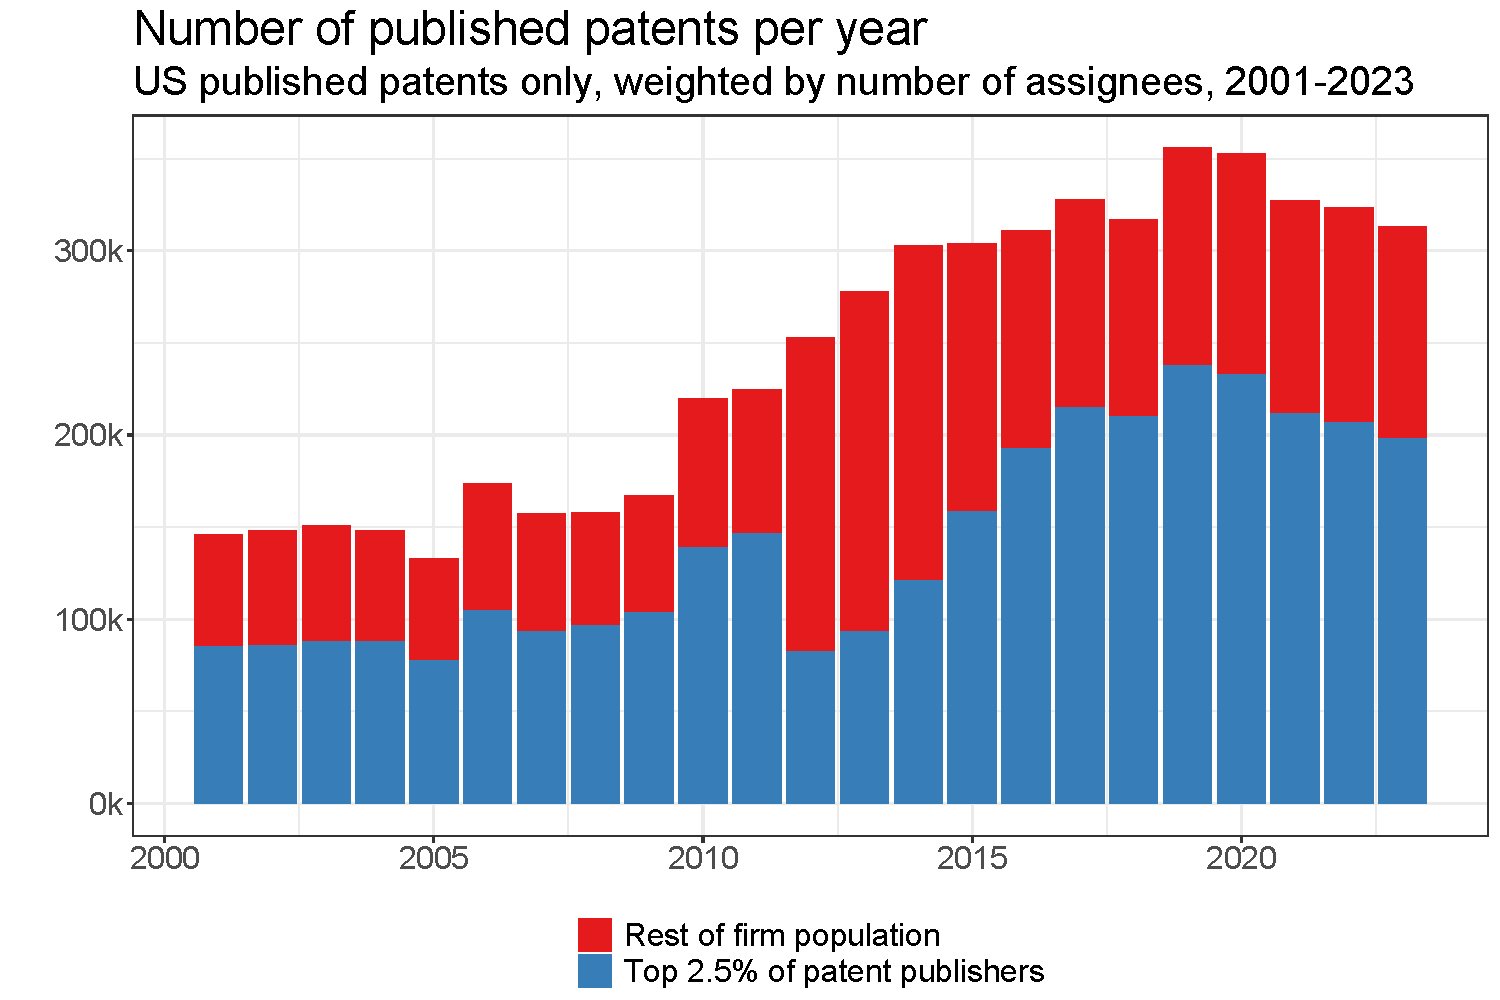
\includegraphics{plot1.pdf}
}
\centering
\end{figure}
Figure 1 shows that the number of patents has increased significantly over the past few decades, more than doubling from 150,000 at the turn of the century to over 300,000 by 2023. Notably, the top 2.5\% of patent publishers represent a major portion of these publications, especially before 2011 and after 2015, when more than half of the patents published came from this group. To simplify computations, this analysis can be restricted to a subset of the largest companies in terms of patent publications. Thanks to the patent concentration, this approach still allows for meaningful commentary on broader trends in the patent markets.

\begin{figure}[h]
\caption{Share of citations per year}
\scalebox{0.6}{
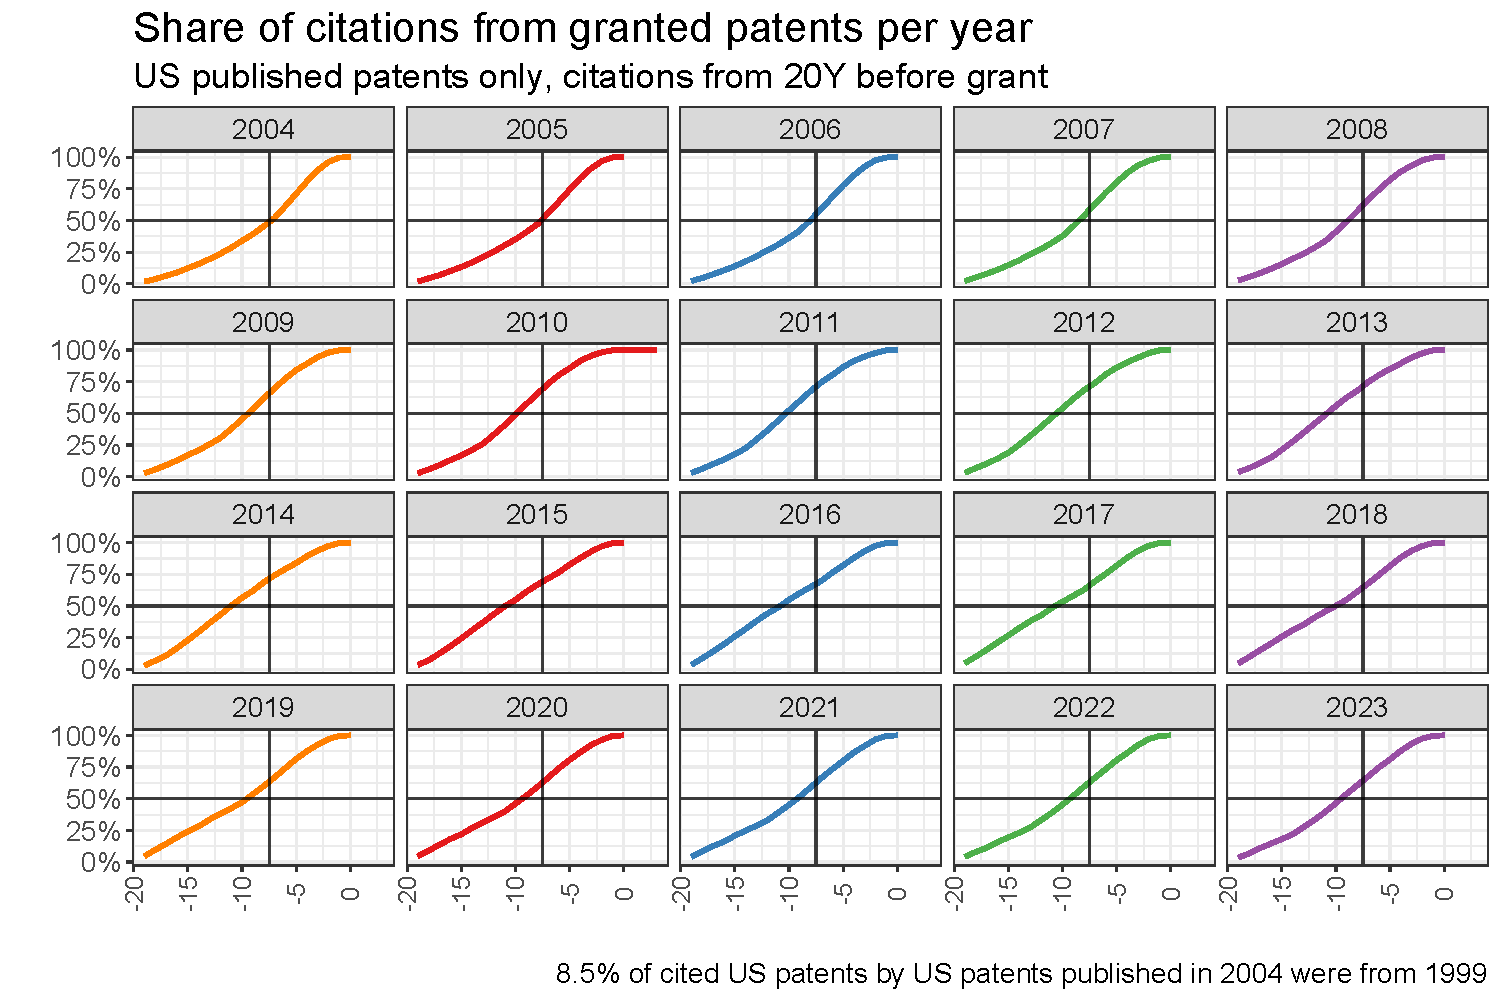
\includegraphics{plot3.pdf}
}
\centering
\end{figure}

Figure 2 presents the cumulative sum of citations given by patents published in a given year. It can be observed that, in the early to mid-2000s, half of the citations were given to patents published in the previous 7.5 years. However, after the Great Financial Crisis, a shift occurred, with more citations being attributed to patents granted earlier than 7.5 years. This shift could indicate that more recent publications remain relevant for a longer time or suggest that more firms are engaging in blocking behaviours, causing the USPTO to cite their patents over longer periods. This result will be used later to model innovation networks using a timeframe closer to the early 2000s citations timeframe.

\begin{figure}[h]
\caption{Share of citations per year}
\scalebox{0.6}{
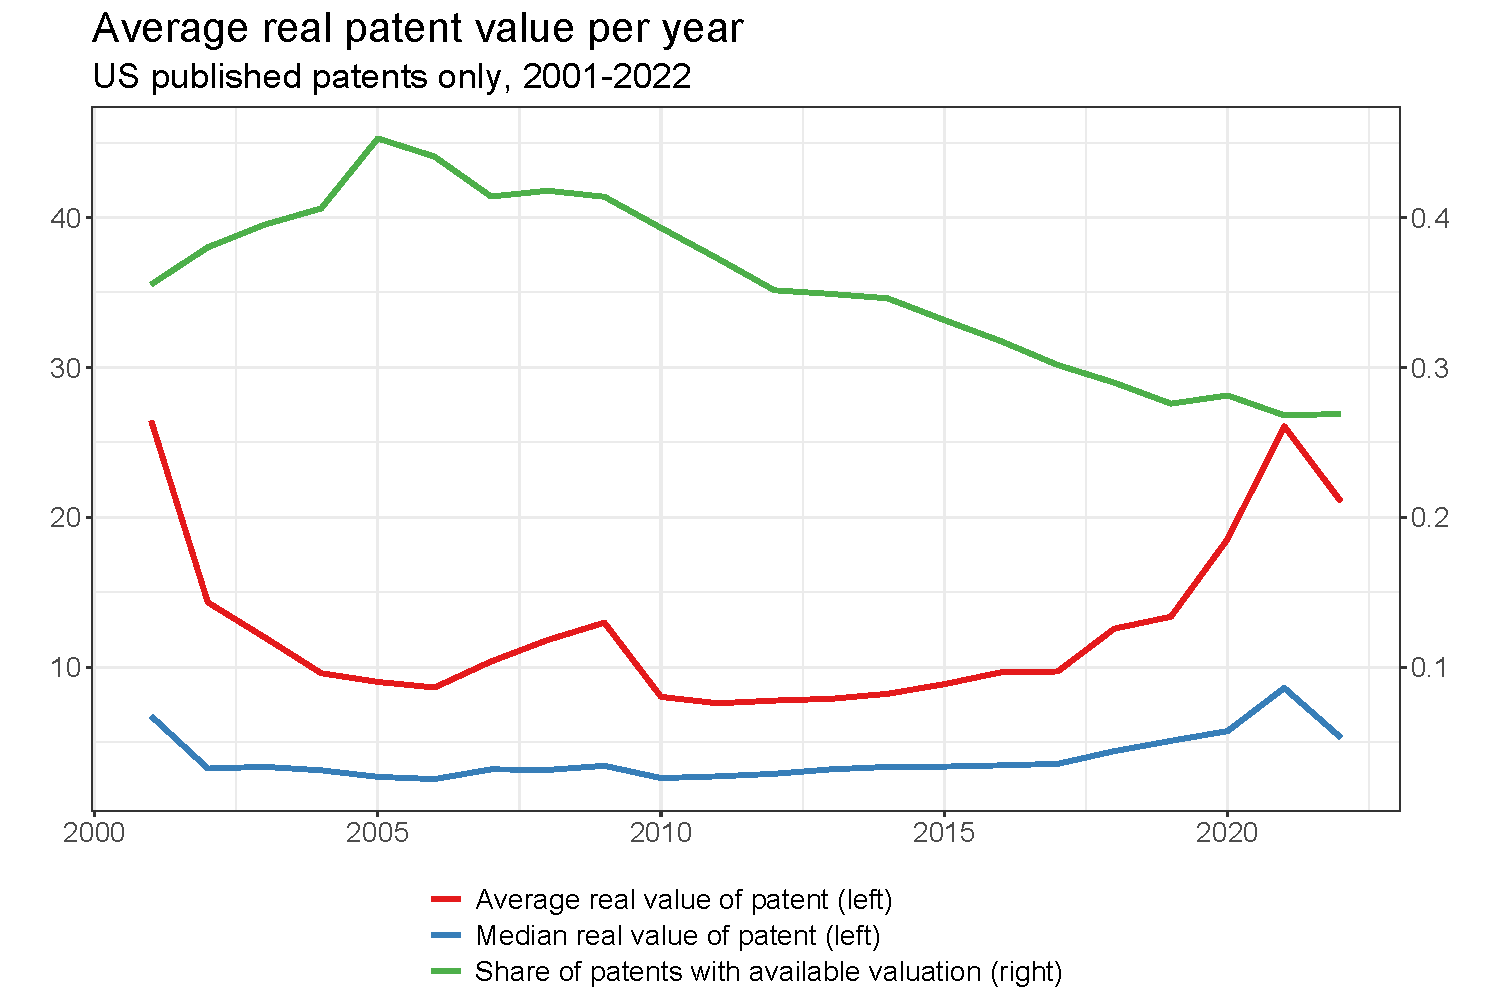
\includegraphics{plot4.pdf}
}
\centering
\end{figure}

Figure 3 has a twofold significance. First, it may reveal the limitations in the work of Kogan et al. Their conclusions and results are partly based on the efficient market theory, which may not hold in practice, leading to the overvaluation of patents during periods of intense financial stress. Three such periods can be identified in the graph: the end of the internet bubble in the early 2000s, the Great Financial Crisis at the end of the 2000s, and the COVID-19 pandemic. When modelling, it will be important to avoid these periods to account for this potential overvaluation.
The second observation from Figure 3 is the decrease in the share of patents granted to publicly traded companies. This trend is related to the overall increase in the number of patents granted, as seen in Figure 1, and is driven by a relative increase in the number of firms publishing one or two patents per year. These smaller entities are less likely to be publicly traded.

\section{Empirical strategy}
The main issue when studying the effects of blocking behaviours by firms is characterising those behaviours. The economic value of a patent cannot be used as a reliable proxy for blocking behaviours, even though blocking patents are often less innovative; they still hold value due to the litigation opportunities they offer. One of the main contributions of this study is to propose a new measure to gauge the degree to which a patent blocks others. This measure will be based on brief behavioural and theoretical arguments and tested in a difference-in-difference framework. It will then be used in conjunction with network modelling to explain the effects of blocking behaviours on the larger network.

\subsection{A New measure of blocking effects}

The situation considered is one with rational agents who anticipate their actions. There are two types of agents: companies, who publish patents when it enables them to improve their profit, and USPTO reviewers who receive patent applications and analyse them before granting the patents or not. 

The additional profit that the publication of the patent can generate is defined as follows:

\[
\Pi = y - c
\]

where $y$ is the additional profit brought about by the patent and $c$ is the cost associated with the patent publication. 

$y$ depends on the innovative value of the patent and on the valuable position that having a patent grants the company. The innovative value of the patent does not change between the application date and the patent issuance date. The value of the position is linked to the number of patents in the network and the differences that exist between the patent considered and the other ones. Hence it is not directly linked to the issuance or not of a patent. 

$c$, as it is anticipated by the company, depends on two elements: the cost of filing a patent application, answering to USPTO requests which utilise human resources and a second cost related to the litigation risk. Let us denote it $r$. $r$ is increasing in the number of existing patents and increasing in the number of would-be patents (that are still wanting approval from the USPTO). 

Yet the risk associated with an application for a patent is smaller than that associated with an actual patent: indeed, there is a chance that an application for a patent is rejected and thus turns out actually not to be risky for the company. That means that the risk associated with an application may turn out to be zero. Let us denote $\rho$ the probability that such a circumstance does not occur, that is to say that a given application is accepted and turned into a patent. Then the above can be rewritten as: $r \equiv r(b_g,\rho b_a)$.

The firm will then choose to apply for a patent if and only if: 
\[
y - r(b_g,\rho b_a) \geq 0
\]
where $\rho < 1$

It is clear that this decision is immediately linked with the probability that competitors' applications are accepted. There is a discontinuity at the time when the applications become actual patents because at that point $b_g$ increases by one and $b_a$ decreases by one. But, as $\rho < 1$, the global effect is an increasing one and as $r$ is increasing in both the variables, it increases. 
The effect of competitors being granted patents may result in a firm considering fewer patent applications or abandoning their current applications. One could argue that the USPTO's decision to grant a patent depends on the status of other similar pending patents (whether published or granted), but legally, this should not be the case. The patent office assesses the novelty of a patent rather than its litigation risk. Novelty is threatened even by pre-grant publications, not just full grants.
Having established this, it is possible to analyse the effect of patent issuance on subsequent innovation by observing the number of citations received.
A second issue is that the granting of a patent increases its visibility, which in turn could increase the number of citations it receives. However, these effects are not likely to be immediate, as filing a patent application takes time.
Therefore, a difference-in-difference (diff-in-diff) framework where one can consider patent applications that are granted at the same date $t_0$. The treatment to examine is the publication of an actual patent. For patent applications submitted at the same time, publication delays may slightly differ: that enables one to define the treatment and the control group. The treatment group is made up of all the patent applications that were granted actual patents at date $t_1$. The control group is made up of all the patent applications that were granted actual patents at date $t_2 > t_1$ (and so that were still applications at $t_1$). Certain dates are particularly convenient to separate these two groups: indeed, because of the holidays, a delay is easily created for patent applications that are examined at that time. These applications are mainly applications that were submitted in September/October. 

\begin{figure}[h]
\caption{Time to publication}
\scalebox{0.6}{
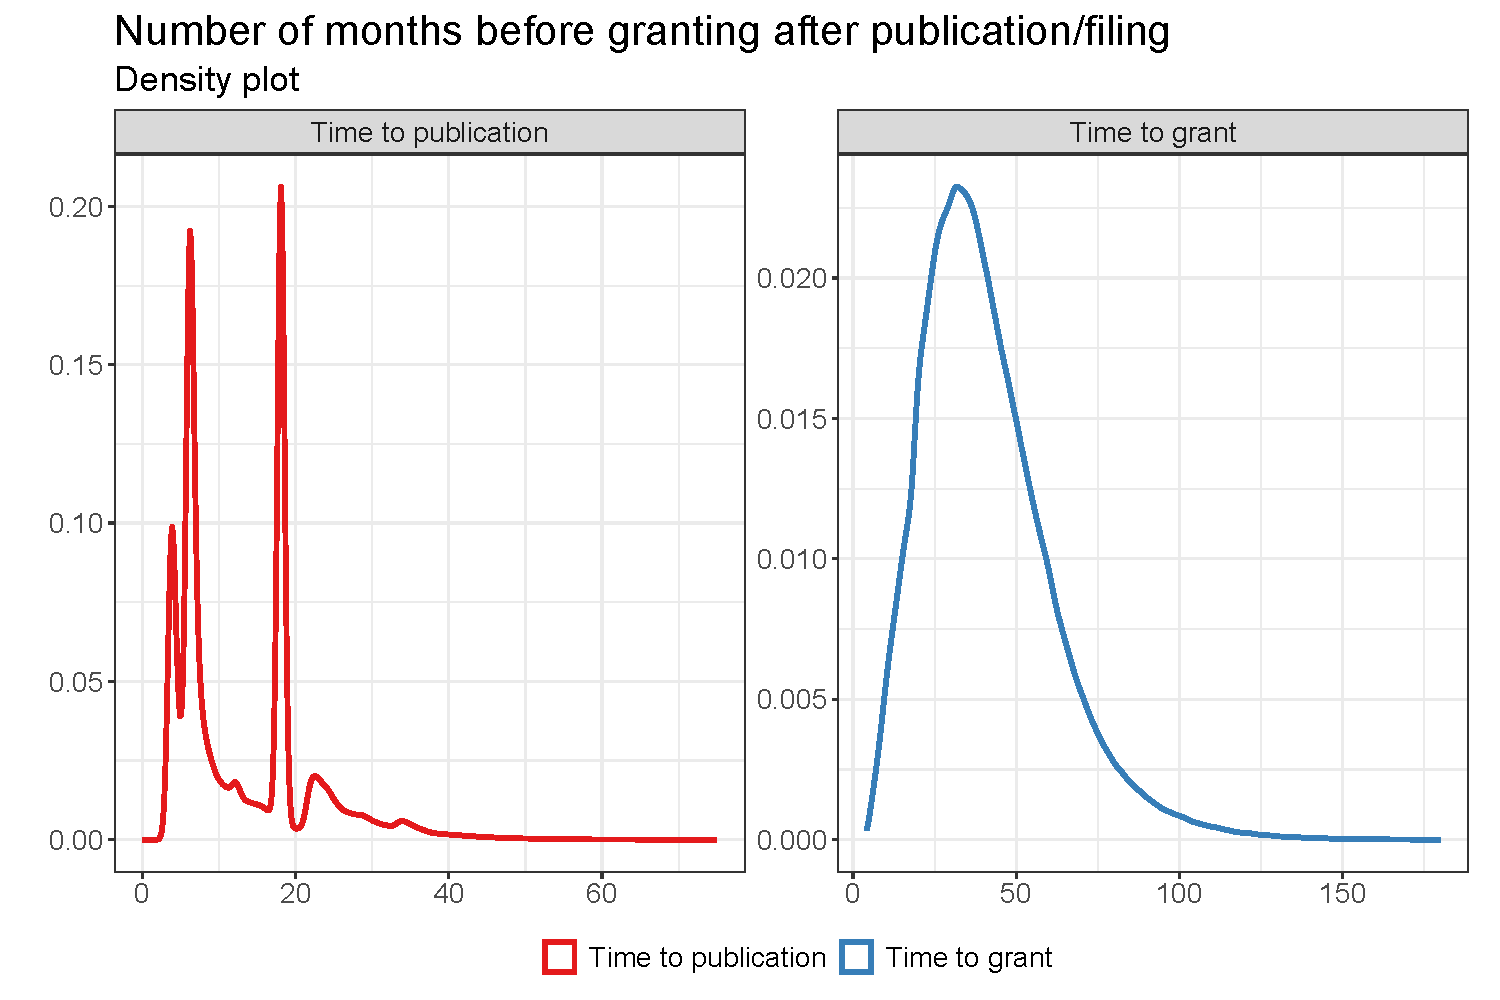
\includegraphics{plot_timings.pdf}
}
\centering
\end{figure}

Based on the distribution of the time to grant it is assumed that a short delay of one quarter is not indicative of differences in patent characteristics but is instead related to external factors (e.g., patent processing being paused for holidays or slowing down during summer when fewer people are working at the USPTO). We selected patents that received their A1 pre-grant publication in a similar timeframe and then received their B2 grant with on average one additional quarter of wait time 7 against 8 quarters. 

\begin{center}
\scalebox{1.2}{
  \tikzfig{tzt}
  }
\hspace*{1.5cm}
\end{center}
We ran this difference-in-difference on two different groups on publication times, and found significant negative effects with a type 2 risk of 5-6%. 
\begin{figure}[h]
\caption{Result of first difference-in-difference}
\scalebox{0.6}{
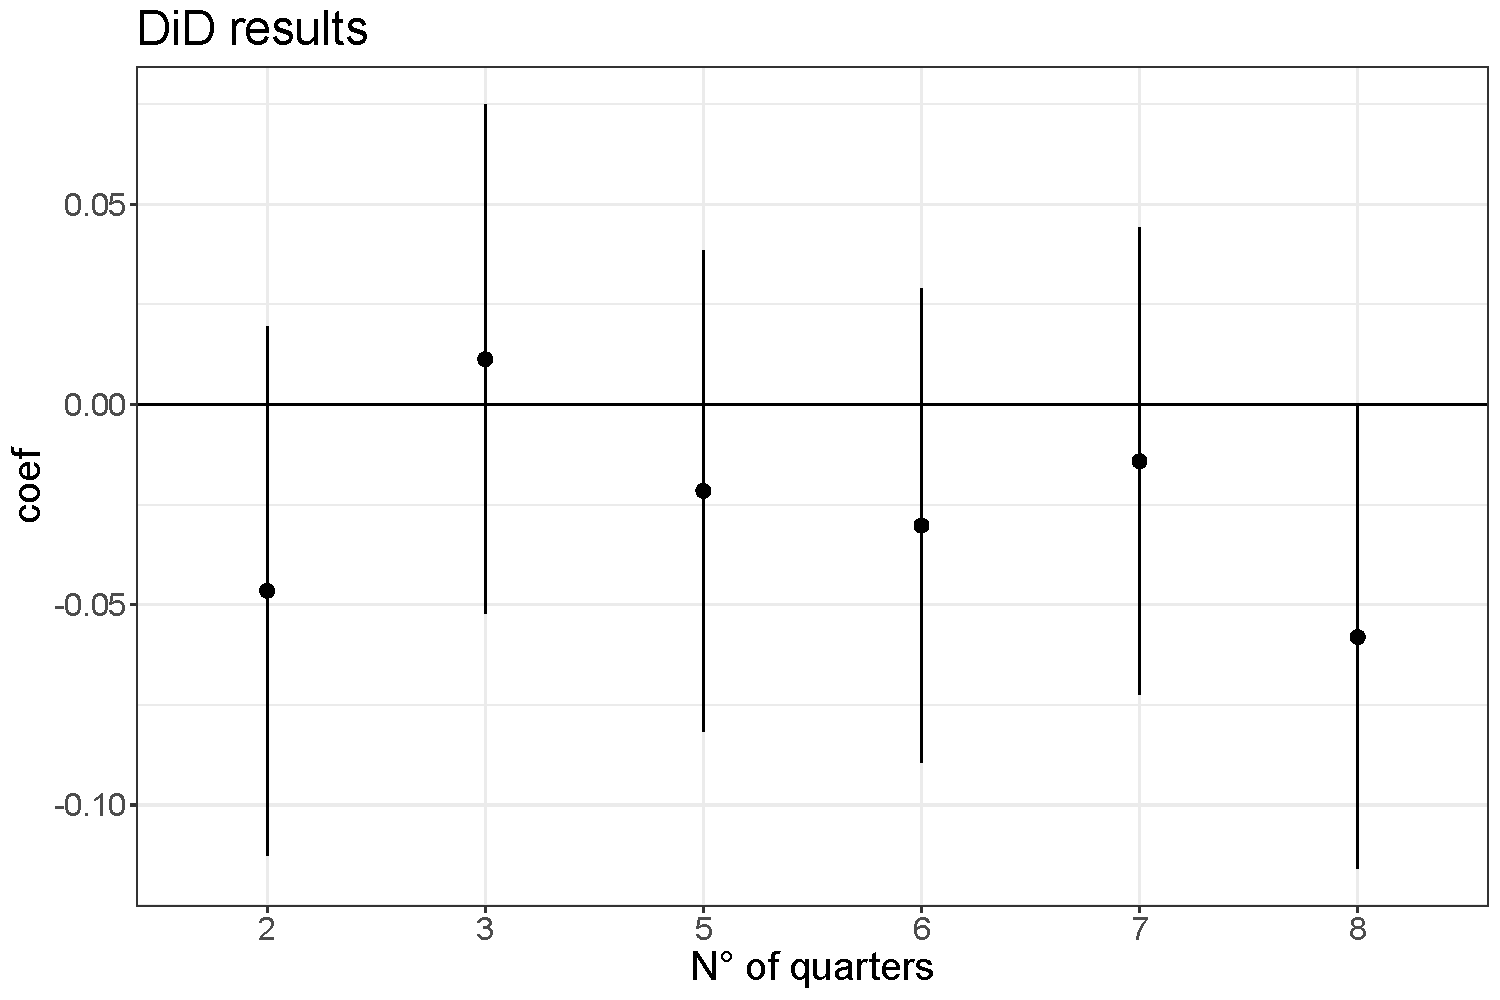
\includegraphics{plotDD1.pdf}
}
\centering
\end{figure}

The full results are annexed to this report, and a visualisation of pretrends is also attached. Those results show that the publication of a patent as B2 (which is to say as an actual patent and not only a mere application) has indeed an effect on the number of subsequent citations. To be precise, the number of subsequent citations stagnates for a while, before increasing a little and decreasing. Now how is that to be analysed thanks to the two effects that have been identified? First the fact that the number of citations increases after a time seems to indicate that there is a positive visibility effect. However, just after the publication of the patent, that positive effect is countered by a negative one: hence the stagnation observed. The citations are searched for in B2 patents so the negative effect in the number of citations corresponds to the fact that, although as many A1 as before cited the patent studied, there are fewer B2 citing it than expected that are actually published. If the number of A1 follows its usual trend before publication, which is what we suppose, this means that, because of the publication of the patent, fewer applications citing it are granted actual patents than what could be expected. Why would this be? It is reasonable to think that, given the publication of the patent, inventors and/or USPTO employees have been deterred from publishing some applications. That can be linked to legal motives (the patents are in fact too similar) or strategic ones (the litigation risks are too high). 

\subsection{Building an innovation network}
To practically test this new measure, it is necessary to construct an innovation network. Given the available data, there are several options for building the innovation network: using patent citations, CPCs (Cooperative Patent Classification), or a similarity measure provided by Google.
The latter offers, for any patent, the closest documents based on content comparisons using machine learning algorithms. While a network built on this measure may help identify different segments of innovation across the market, it provides no insight into firms' strategies. Similarly, a network based on CPCs, though useful for understanding which firms compete in which markets, does not shed light on strategic behaviours.
On the other hand, forward citations can be quite useful. Patent citations can reflect various relationships: citing similar inventions as relevant examples of prior art or citing blocking and defensive patents that are less directly linked to the innovation segment but are general and could lead to litigation. Building the network based on these citations allows for consideration of firms' strategies. This is because the number of citations a patent receives is correlated with the number of patents a firm holds. Deciding to patent extensively or not is a key component of a company's patent strategy.
The network was ultimately built upon the number of forward citations received within five years following which in regards to part II seems sufficient a patent's publication date, limited to the 2.5% of most active patent publishers, the network was constructed twice, avoiding periods of financial stress.

\subsection*{Defining a centrality measure}
Defining a centrality measures 
To identify the most influential companies in innovation transmission and strategy within each cluster, it is necessary to assess the importance of each company using a centrality measure. Two centrality measures were considered: betweenness centrality and closeness centrality.
Companies with high betweenness centrality are crucial for connectivity and effective communication between different parts of the network. This measure counts the number of times a firm lies on the shortest path between two other firms, highlighting its role in linking disparate network segments. On the other hand, closeness centrality measures the ability of a node to rapidly disseminate information throughout the network, identifying firms that can quickly influence the entire network.
Since the size of the links does not significantly impact betweenness centrality, it will primarily be used for regressions at the company level. Conversely, closeness centrality will be useful for regressions involving cluster-level variables, allowing for weighting the importance of all network components. This approach ensures that both individual and collective influences within the innovation network are adequately captured and analysed.

\subsection{Regressions}
Once these tools are designed, it is possible to turn to the analysis of correlation between the variables, that will be conducted through several regressions. A series of regressions has been conducted for patents published between 2005 and 2007 and then for patents published between 2013 and 2015. 

First, real patent value was regressed on centrality, the difference between the number of citations of a patent after and before its publication as a B2 patent (the custom measure proposed by this project hereafter called Delta), the number of CPCs of the firm, the number of patents published by the firm and the similarity share. The similarity share is the proportion, among all the citations of patent X, of citations that come from patents identified as “similar” to X (the identification is based on Google measure of similarity). 

Then, centrality was regressed on patent value, Delta and the number of patents published by the firm. 

Finally, the number of patents some years after (2015 for 2003-2005 patents and 2019 for 2013-2015 patents) was regressed on centrality, the number of patents published, the similarity share, the number of CPCs, patent value and Delta. The aim is to see how relevant these values are to predict future patenting. 

\section{Results}
\subsection{Correlations}
The following regression aimed at understanding the correlations between patent value and different variables. Given the previous result, it seems logical to include Delta (the difference in the number of citations before and after the patent publication) in the regression. Moreover, as explained above, a patent value has both an innovative and a strategic value: that means that citations may stem from similarities in the patents or from the fact that a patent is “blocking”. So it is interesting to take into account what proportion of the citations come from similar patents, as that can give insight into the nature of the patent. Hence, patent value (in log) was regressed on centrality, number of CPCs linked to the patent, Delta and the similarity share that corresponds to the part of similar citing patents. The output of the regression shows no significant coefficient for the 2005-2005 period but for the other period, share of similar citations and delta have a positive effect on the patent value. 
The lack of significance for the first period can be attributed to the fewer number of companies publishing during that time. Consequently, the top 2.5\% that constitutes our sample contains fewer companies. Since the p-value can be viewed as a decreasing function of n (sample size), it is normal for the coefficients to not be significant. A big proportion of similar patents among the citing patents can be seen as a signal of innovative patents within their field, thus being valued by the market. This highlights an offensive strategy. The delta value indicates a potential blocking strategy because the publication of a blocking patent aims to discourage others from pursuing their own publications. Thus, blocking other entities in their innovation can enhance the value of the patent, especially if it holds the power to litigate against rivals.


\begin{table}[h!]
\centering
\caption{Regression Results for 2013:2015 and 2005:2007}
\label{tab:regression_comparison}
\begin{tabular}{lcccc}
\toprule
 & \multicolumn{2}{c}{\textbf{2013:2015}} & \multicolumn{2}{c}{\textbf{2005:2007}} \\
\cmidrule(lr){2-3} \cmidrule(lr){4-5}
\textbf{Variable} & \textbf{Estimate} & \textbf{Pr($>|$t$|$)} & \textbf{Estimate} & \textbf{Pr($>|$t$|$)} \\
\midrule
\textbf{PatentVal} & & & & \\
Intercept         & 2.735e+00 & $<2e-16^{***}$ & 2.346e+00 & 0.000123$^{***}$ \\
Bet Centrality         & 9.021e-05 & 0.024235$^{*}$ & 3.061e-04 & 0.144087 \\
DeltaB2                & 1.576e-02 & 0.000138$^{***}$ & -2.895e-02 & 0.516120 \\
N. of CPC           & -3.712e-03 & 0.095035$^{.}$ & -9.938e-03 & 0.091423$^{.}$ \\
Sim Share         & -8.489e-03 & 0.000110$^{***}$ & -5.461e-02 & 0.475704 \\
N. of pub patents              & -7.689e-05 & 0.040475$^{*}$ & -9.915e-05 & 0.322615 \\
\midrule
\multicolumn{1}{l}{\textbf{Residual Std. Error:}} & \multicolumn{2}{c}{0.9695} & \multicolumn{2}{c}{1.202} \\
\multicolumn{1}{l}{\textbf{Degrees of Freedom:}} & \multicolumn{2}{c}{2805} & \multicolumn{2}{c}{429} \\
\multicolumn{1}{l}{\textbf{Multiple R-squared:}} & \multicolumn{2}{c}{0.2097} & \multicolumn{2}{c}{0.2738} \\
\multicolumn{1}{l}{\textbf{Adjusted R-squared:}} & \multicolumn{2}{c}{0.1891 } & \multicolumn{2}{c}{0.201 } \\
\multicolumn{1}{l}{\textbf{F-statistic:}} & \multicolumn{2}{c}{10.19} & \multicolumn{2}{c}{3.762} \\
\multicolumn{1}{l}{\textbf{P-value:}} & \multicolumn{2}{c}{2.2e-16} & \multicolumn{2}{c}{9.322e-13} \\
\midrule
\textbf{Centrality (Robust)} & & & & \\
Intercept         & 1.831e+00 & 8.41e-09$^{***}$ & 1.888e+00 & 0.005478$^{**}$ \\
Patent Real Value          & 5.062e-03 & 0.03217$^{*}$ & 9.009e-03 & 0.000503$^{***}$ \\
DeltaB2              & 3.305e-02 & 7.24e-05$^{***}$ & -6.485e-03 & 0.897153 \\
N. of pub patents               & 7.128e-04 & $<2e-16^{***}$ & 6.055e-04 & $<2e-16^{***}$ \\
Cluster size       & 9.714e-03 & $<2e-16^{***}$ & 8.688e-03 & $<2e-16^{***}$ \\
\midrule
\multicolumn{1}{l}{\textbf{Residual Std. Error:}} & \multicolumn{2}{c}{1.941} & \multicolumn{2}{c}{1.351} \\
\multicolumn{1}{l}{\textbf{Degrees of Freedom:}} & \multicolumn{2}{c}{2806} & \multicolumn{2}{c}{430} \\
\multicolumn{1}{l}{\textbf{Multiple R-squared:}} & \multicolumn{2}{c}{0.398} & \multicolumn{2}{c}{0.5653} \\
\multicolumn{1}{l}{\textbf{Adjusted R-squared:}} & \multicolumn{2}{c}{0.3826} & \multicolumn{2}{c}{0.5229} \\
\multicolumn{1}{l}{\textbf{F-statistic:}} & \multicolumn{2}{c}{25.77} & \multicolumn{2}{c}{13.32} \\
\multicolumn{1}{l}{\textbf{P-value:}} & \multicolumn{2}{c}{2.2e-16} & \multicolumn{2}{c}{ 2.2e-16} \\
\bottomrule
\end{tabular}
\end{table}

Then centrality was regressed on patent value, Delta and the number of patents published the same year. The errors showed heterosexuality so a robust option was used.  The number of patents published has a significant and positive coefficient. So the more patents a firm publishes during a period and the more central it is in the network. That can be explained by the fact that publishing many patents is often associated with defensive patent strategies. As defensive strategies aim at blocking competitors as much as possible, firms that resort to these strategies will most probably try to publish patents in as many fields as possible, in order to block as many competitors as possible and to be in the position to demand royalties. If the blocking is effective then the position of the company becomes more intermediate in the cluster therefore the centrality increases. 

\subsection{Impact on future patent publications}

In order to explain the number of patents published by a company, a regression was conducted, of the number of publications in 2015 for the 2005-2007 period and in 2019 for the 2013-1015 period, on the centrality of the firm within its sub-network (measured by betweenness centrality), and the number of patents published during the considered period. For both periods, the number of technological sectors associated with the patent (ncpc), the real value and centrality have a positive effect. The part of similar citations has a negative impact. 

By comparing with the same regression at the cluster level, we find that ncpc$\times$centrality has a positive coefficient. Therefore, being centrally positioned within one's cluster and publishing a patent that spans more sectors leads to an increase in the number of publications in 2019. It is plausible that a patent spanning multiple sectors is of a defensive nature. Besides, at the cluster level, Delta has a negative effect but the number of published patents NPP$\times$Delta has a positive impact. Thus, the strategy that aims at blocking competition appears to benefit the most central and the biggest companies more than the others, owing to their strong influence in innovation transmission. 


\begin{table}[h!]
\centering
\caption{Detailed Regression Results for Different Periods}
\label{tab:regression_results}
\begin{tabular}{lcccc}
\toprule
\textbf{Dependant variable} & \multicolumn{2}{c}{\textbf{2013:2015}} & \multicolumn{2}{c}{\textbf{2005:2007}} \\
\midrule
\textbf{N° Patents after 5y (resp. 2015)} & \textbf{Estimate} & \textbf{Pr($>|$t$|$)} & \textbf{Estimate} & \textbf{Pr($>|$t$|$)} \\
\midrule
Intercept          & 1.019e+00 & 1.30e-05*** & 2.882e+00 & 0.001878** \\
Bet Centrality          & 7.062e-04 & $<$2e-16***   & 1.070e-03 & 0.001215** \\
N. of pub patents                  & -1.892e-04 & 9.96e-05*** & 9.066e-05 & 0.557378 \\
Sim Share           & -2.248e-02 & 3.57e-15*** & -1.017e+00 & $<$2e-16*** \\
N. of CPC             & 1.014e-01 & $<$2e-16***   & 3.698e-02 & 0.000175*** \\
Patent Real Value            & 8.364e-03 & 4.81e-08*** & 1.144e-02 & 0.002039** \\
DeltaB2                  & 1.492e-02 & 0.094583    & -2.102e-03 & 0.984051 \\
\midrule
\multicolumn{1}{l}{\textbf{Residual Std. Error:}} & \multicolumn{2}{c}{1.254} & \multicolumn{2}{c}{1.801} \\
\multicolumn{1}{l}{\textbf{Degrees of Freedom:}} & \multicolumn{2}{c}{2803} & \multicolumn{2}{c}{407} \\
\multicolumn{1}{l}{\textbf{Multiple R-squared:}} & \multicolumn{2}{c}{0.4352} & \multicolumn{2}{c}{0.2738} \\
\multicolumn{1}{l}{\textbf{Adjusted R-squared:}} & \multicolumn{2}{c}{0.345} & \multicolumn{2}{c}{0.201 } \\
\multicolumn{1}{l}{\textbf{F-statistic:}} & \multicolumn{2}{c}{4.824} & \multicolumn{2}{c}{3.762} \\
\multicolumn{1}{l}{\textbf{P-value:}} & \multicolumn{2}{c}{$<$2.2e-16} & \multicolumn{2}{c}{$<$2.2e-16} \\
\midrule
\textbf{N° Patents after 5y (resp. 2015)} & & & & \\
Intercept          & 7.2406e-01 & 2.2e-16***  & 1.5591e+00 & 0.0007026*** \\
N. of pub patents (Npp)    & 1.9586e-03 & 0.002209**    & 1.2078e-02 & 8.417e-06*** \\
MeanPf Clust            & 1.4198e-02 & 0.380477   & 7.1549e-01 & 0.3817351 \\
Cluster size                 & 1.6998e-03 & 8.081e-07***    & 4.0294e-03 & 0.0003210*** \\
N. of CPC Clust                 & -4.4907e-01 & 0.319823    & -4.0974e+00 & 0.5015621 \\
DeltaB2 Clust                 & -1.0733e+00 & 2.108e-05***    & -1.1718e-02 & 0.0057161** \\
Npp$\times$MeanPf Clust            & -2.2806e-04 & 0.066439.   & -4.5695e+01 & 0.0097960*** \\
Npp$\times$Cluster size       & -2.9982e-06 & 0.029637*   & -2.121e-05 & 4.265e-05*** \\
Npp$\times$N. of CPC Clust           & 7.4327e-03 & 0.031628* & 8.373e-02 & 0.0135016* \\
Npp$\times$DeltaB2 Clust            & 1.3611e-02 & 0.007229* & 1.669e-01 & 0.0516056. \\
\midrule
\multicolumn{1}{l}{\textbf{Residual Std. Error:}} & \multicolumn{2}{c}{1.533} & \multicolumn{2}{c}{2.086} \\
\multicolumn{1}{l}{\textbf{Degrees of Freedom:}} & \multicolumn{2}{c}{2574} & \multicolumn{2}{c}{383} \\
\multicolumn{1}{l}{\textbf{Multiple R-squared:}} & \multicolumn{2}{c}{0.3234} & \multicolumn{2}{c}{0.1805} \\
\multicolumn{1}{l}{\textbf{Adjusted R-squared:}} & \multicolumn{2}{c}{0.321} & \multicolumn{2}{c}{0.1612} \\
\multicolumn{1}{l}{\textbf{F-statistic:}} & \multicolumn{2}{c}{136.7} & \multicolumn{2}{c}{9.373} \\
\multicolumn{1}{l}{\textbf{P-value:}} & \multicolumn{2}{c}{$<$2.2e-16} & \multicolumn{2}{c}{6.578e-13} \\
\bottomrule
\end{tabular}
\end{table}


\section{Conclusion}
On the whole, this study of patent data enables one to understand better the impact of firms’ strategies on innovation. Patent strategies can be analysed through several angles: the number of patents published, the offensive or defensive aspect of these patents and the vast or specific span of these patents. 
A global trend can be observed, that more and more patents are published by more and more companies, which is an indication that patents are taken into account in fims’ strategies more than they were before. However, a large majority of companies only publish very few patents, so in these cases, there is no real patent strategy (firms publish patents when they really innovate), contrary to big companies. 
The analysis conducted here underlines the role of the blocking aspects of patents. This blocking characteristic has a negative impact on innovation. Indeed, the publication of a patent implies that inventors who want to further develop this innovation will either have to pay royalties or expose themselves to possible litigation. Yet, the bigger the company considered, the smaller this negative impact is. So patent strategies have a higher impact on small firms than on big ones. That is something to bear in mind when conducting patent policies, as it can help to design adequate measures to counter these blocking strategies. 
Furthermore, as time goes by, more and more citations come from patents published long before. Patents tend to cite older references than they used to. That is also an indication. There are two reasons for citing a patent: either because it is related to an innovation that one has carried further or because it is a blocking patent and that not citing it may be a cause for litigation. On the innovation level, patents are often related to other patents that were published not long before. So this change of trend is most probably a sign of a global change in patent strategies, which are becoming more blocking than before. It is consistent with the increase in the number of patents, which indicates the same change in strategies. 
One limitation of the model here is that, in analysing the impact of strategies over innovation, innovation has been measured through the number of patents. And this is not quite accurate because some patents are more innovative than others. However, all the patents are at least slightly innovative (else they would be rejected by the USPTO) so the results are significant. 
To further explore this question of defensiveness of patents, one could rely on the Delta measured above (the difference between citations after and before B2 publication) and compare it with the significance measure of a patent that was developed by Kelly et al. (“Measuring technological innovation over the long run”). Indeed, Delta measures the defensiveness of a patent, Kelly measures the novelty of a patent, and these two elements are the main characteristics to consider when trying to define a patent value. It may then be interesting to work on how they interact and how they may be tackled more efficiently by economic policies. 
\newpage

\section{References}
Kogan, L., Papanikolaou, D., Seru, A., \& Stoffman, N. (2017), “Technological innovation, resource allocation and growth”, The Quarterly Journal of Economics, 132(2), 665-712.

Kelly, B., Papanikolaou, D., Seru, A., \& Taddy, M. (2018), “Measuring technological innovation over the long run”, American Economic Review: Insights, 3(3), 303-320.

Acemoglu, D., Akcigit, U., \& Kerr, W. (2016), “Innovation network”, Proceedings of the National Academy of Sciences, 113(41), 11483-11488.

Traag, V. A., \& Waltman, L. (2018), “From Louvain to Leiden: guaranteeing well-connected communities”, Scientific reports

REITZIG M., “The private values of ‘thickets’ and ‘fences’: towards an updated picture of the use of patents across industries”, The Economics of Innovation and New Technology, vol. 13, n° 5, July, pp. 457-476 (2004)

CORBEL. P., “Le brevet : un instrument d’équilibration stratégique”, Association Internationale de Management Stratégique (2004)
\newpage

\section{Annexes}
\begin{table}[h!]
\centering
\caption{Annex1: DiD Results}
\label{tab:regression_comparison}
\begin{tabular}{lcccc}
\toprule
 & \multicolumn{2}{c}{\textbf{Model 1 (Data1)}} & \multicolumn{2}{c}{\textbf{Model 2 (Data2)}} \\
\cmidrule(lr){2-3} \cmidrule(lr){4-5}
\textbf{Variable} & \textbf{Estimate} & \textbf{Pr($>|$t$|$)} & \textbf{Estimate} & \textbf{Pr($>|$t$|$)} \\
\midrule
Intercept         & 0.6587 & $<2e-16^{***}$ & 0.7029 & $<2e-16^{***}$ \\
quarter2          & 0.0034 & 0.8906 & -0.0356 & 0.0393$^{*}$ \\
quarter3          & -0.0144 & 0.5401 & -0.0387 & 0.0173$^{*}$ \\
quarter4          & -      & -     & -0.0296 & 0.0616$^{.}$ \\
quarter5          & 0.0425 & 0.0568$^{.}$ & -      & - \\
quarter6          & 0.0414 & 0.0617$^{.}$ & -0.0135 & 0.3741 \\
quarter7          & 0.0253 & 0.2466 & -0.0112 & 0.4503 \\
quarter8          & 0.0460 & 0.0334$^{*}$ & 0.0131 & 0.3769 \\
Treated           & 0.0169 & 0.4677 & 0.0032 & 0.8364 \\
quarter2$\times$Treated & -0.0465 & 0.1857 & 0.0045 & 0.8548 \\
quarter3$\times$Treated & 0.0113 & 0.7371 & -0.0110 & 0.6367 \\
quarter4$\times$Treated & -      & -     & -0.0188 & 0.4040 \\
quarter5$\times$Treated & -0.0216 & 0.4982 & -      & - \\
quarter6$\times$Treated & -0.0302 & 0.3366 & -0.0180 & 0.4025 \\
quarter7$\times$Treated & -0.0141 & 0.6480 & -0.0092 & 0.6624 \\
quarter8$\times$Treated & -0.0580 & 0.0587$^{.}$ & -0.0411 & 0.0499$^{*}$ \\
\midrule
\multicolumn{1}{l}{\textbf{Residual Std. Error:}} & \multicolumn{2}{c}{0.6267} & \multicolumn{2}{c}{0.6308} \\
\multicolumn{1}{l}{\textbf{Degrees of Freedom:}} & \multicolumn{2}{c}{22338} & \multicolumn{2}{c}{44854} \\
\multicolumn{1}{l}{\textbf{Multiple R-squared:}} & \multicolumn{2}{c}{0.001056} & \multicolumn{2}{c}{0.0007732} \\
\multicolumn{1}{l}{\textbf{Adjusted R-squared:}} & \multicolumn{2}{c}{0.0004743} & \multicolumn{2}{c}{0.0004836} \\
\multicolumn{1}{l}{\textbf{F-statistic:}} & \multicolumn{2}{c}{1.816} & \multicolumn{2}{c}{2.67} \\
\multicolumn{1}{l}{\textbf{P-value:}} & \multicolumn{2}{c}{0.03501} & \multicolumn{2}{c}{0.000941} \\
\bottomrule
\end{tabular}
\end{table}

\begin{figure}[h]
\caption{Diff-in-diff 1: Pretrends}
\scalebox{0.6}{
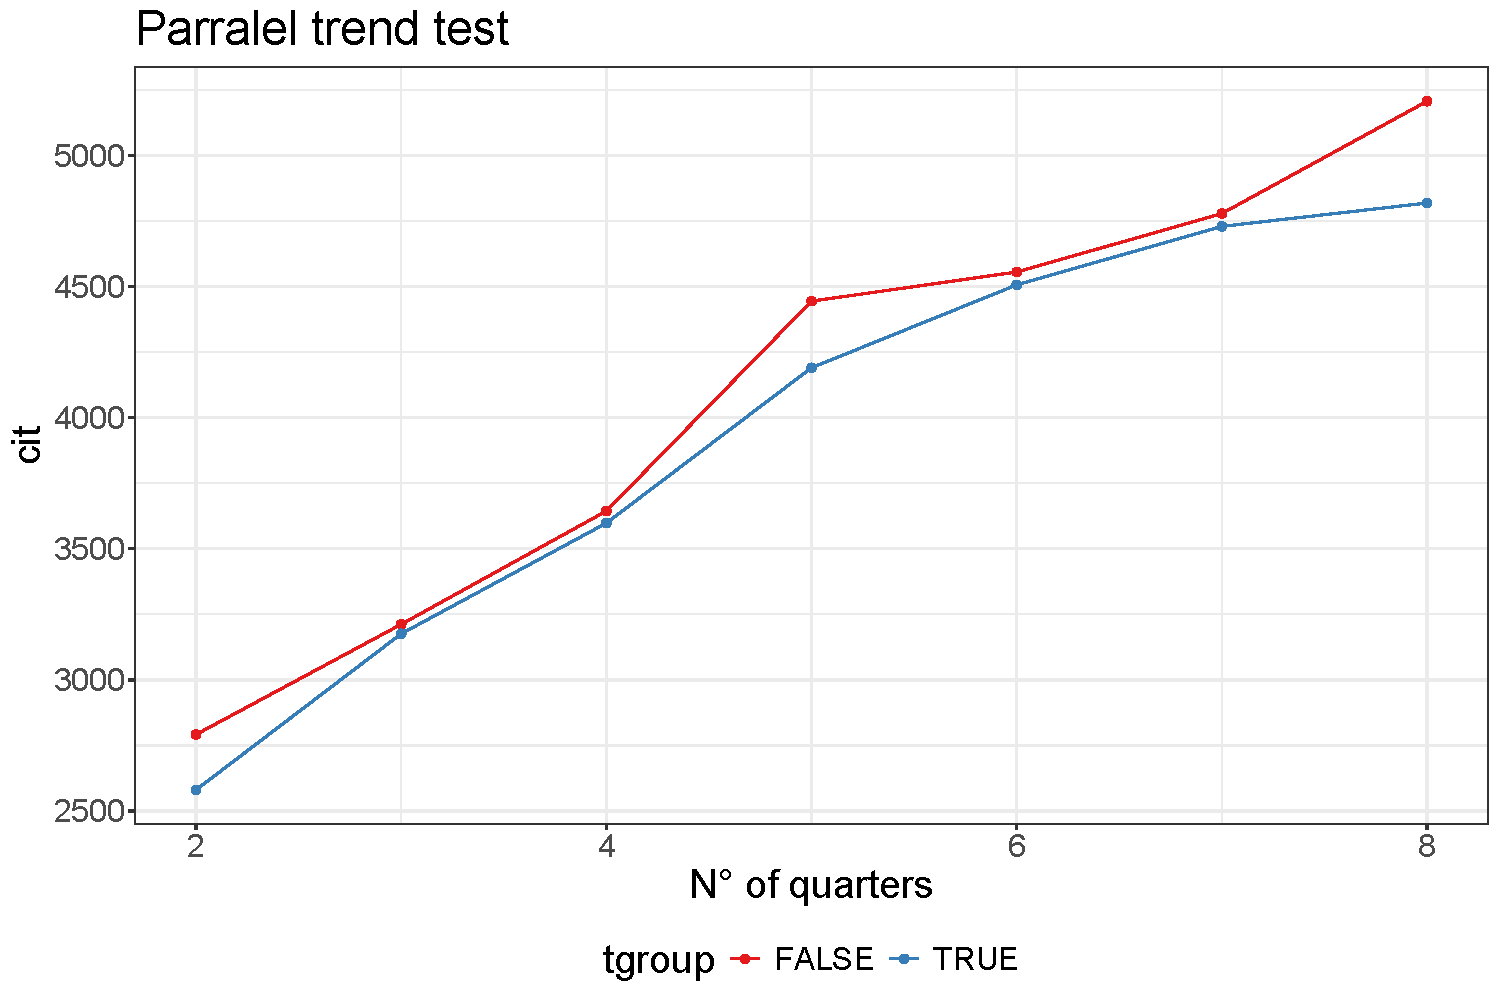
\includegraphics{ptrend1.pdf}
}
\centering
\end{figure}

\begin{figure}[h]
\caption{Diff-in-diff 2: Pretrends}
\scalebox{0.6}{
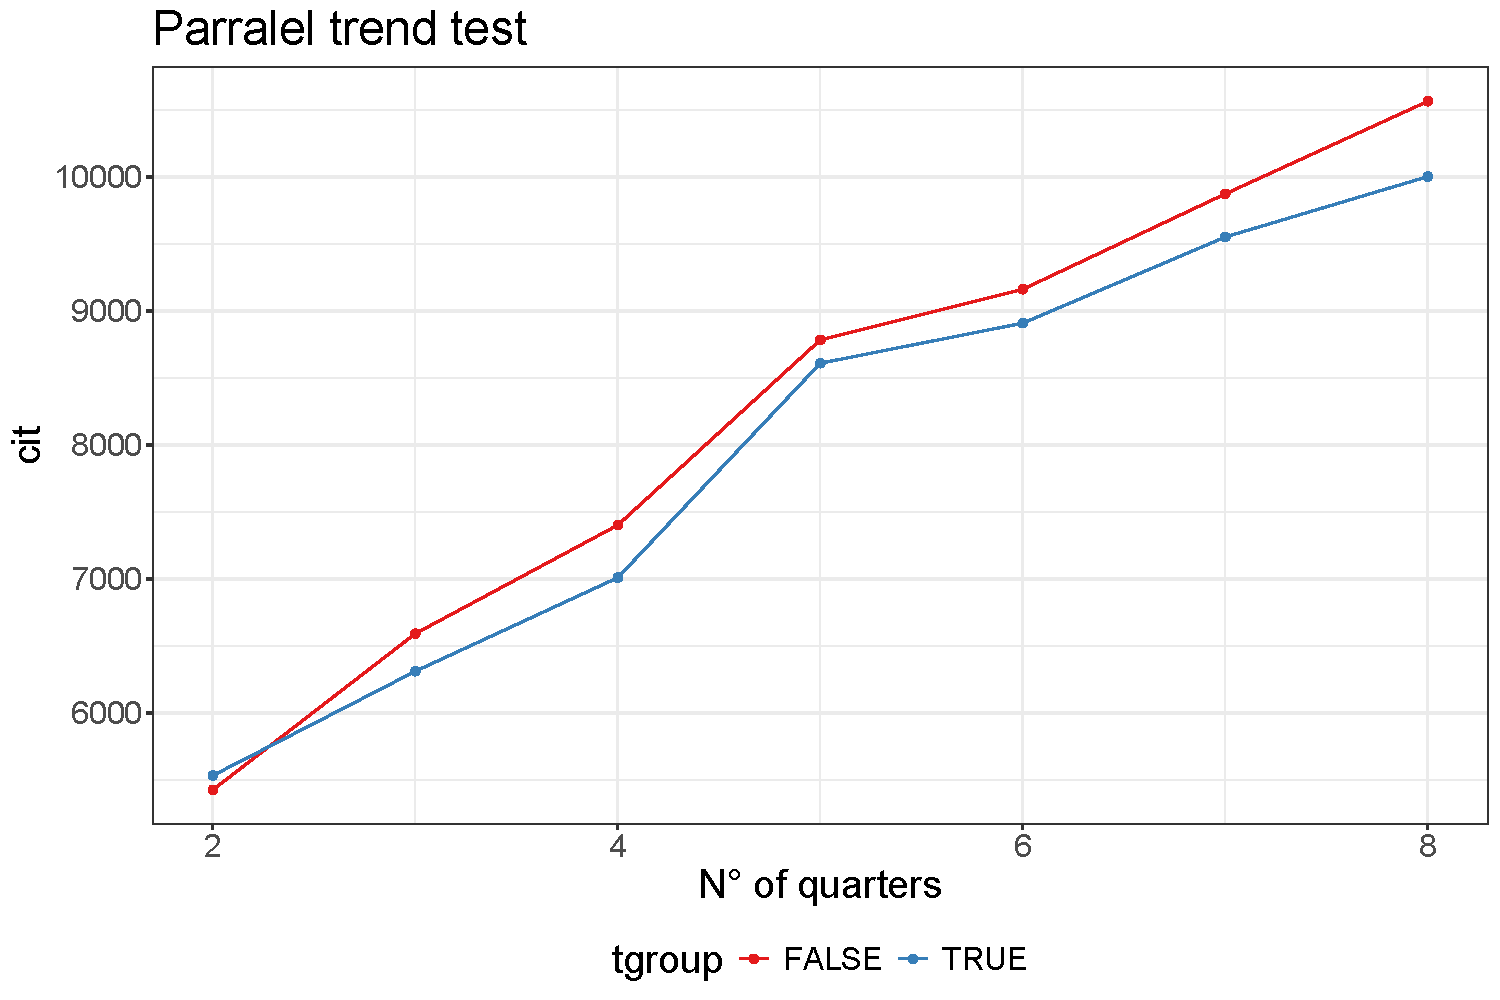
\includegraphics{ptrend2.pdf}
}
\centering
\end{figure}

\newpage 

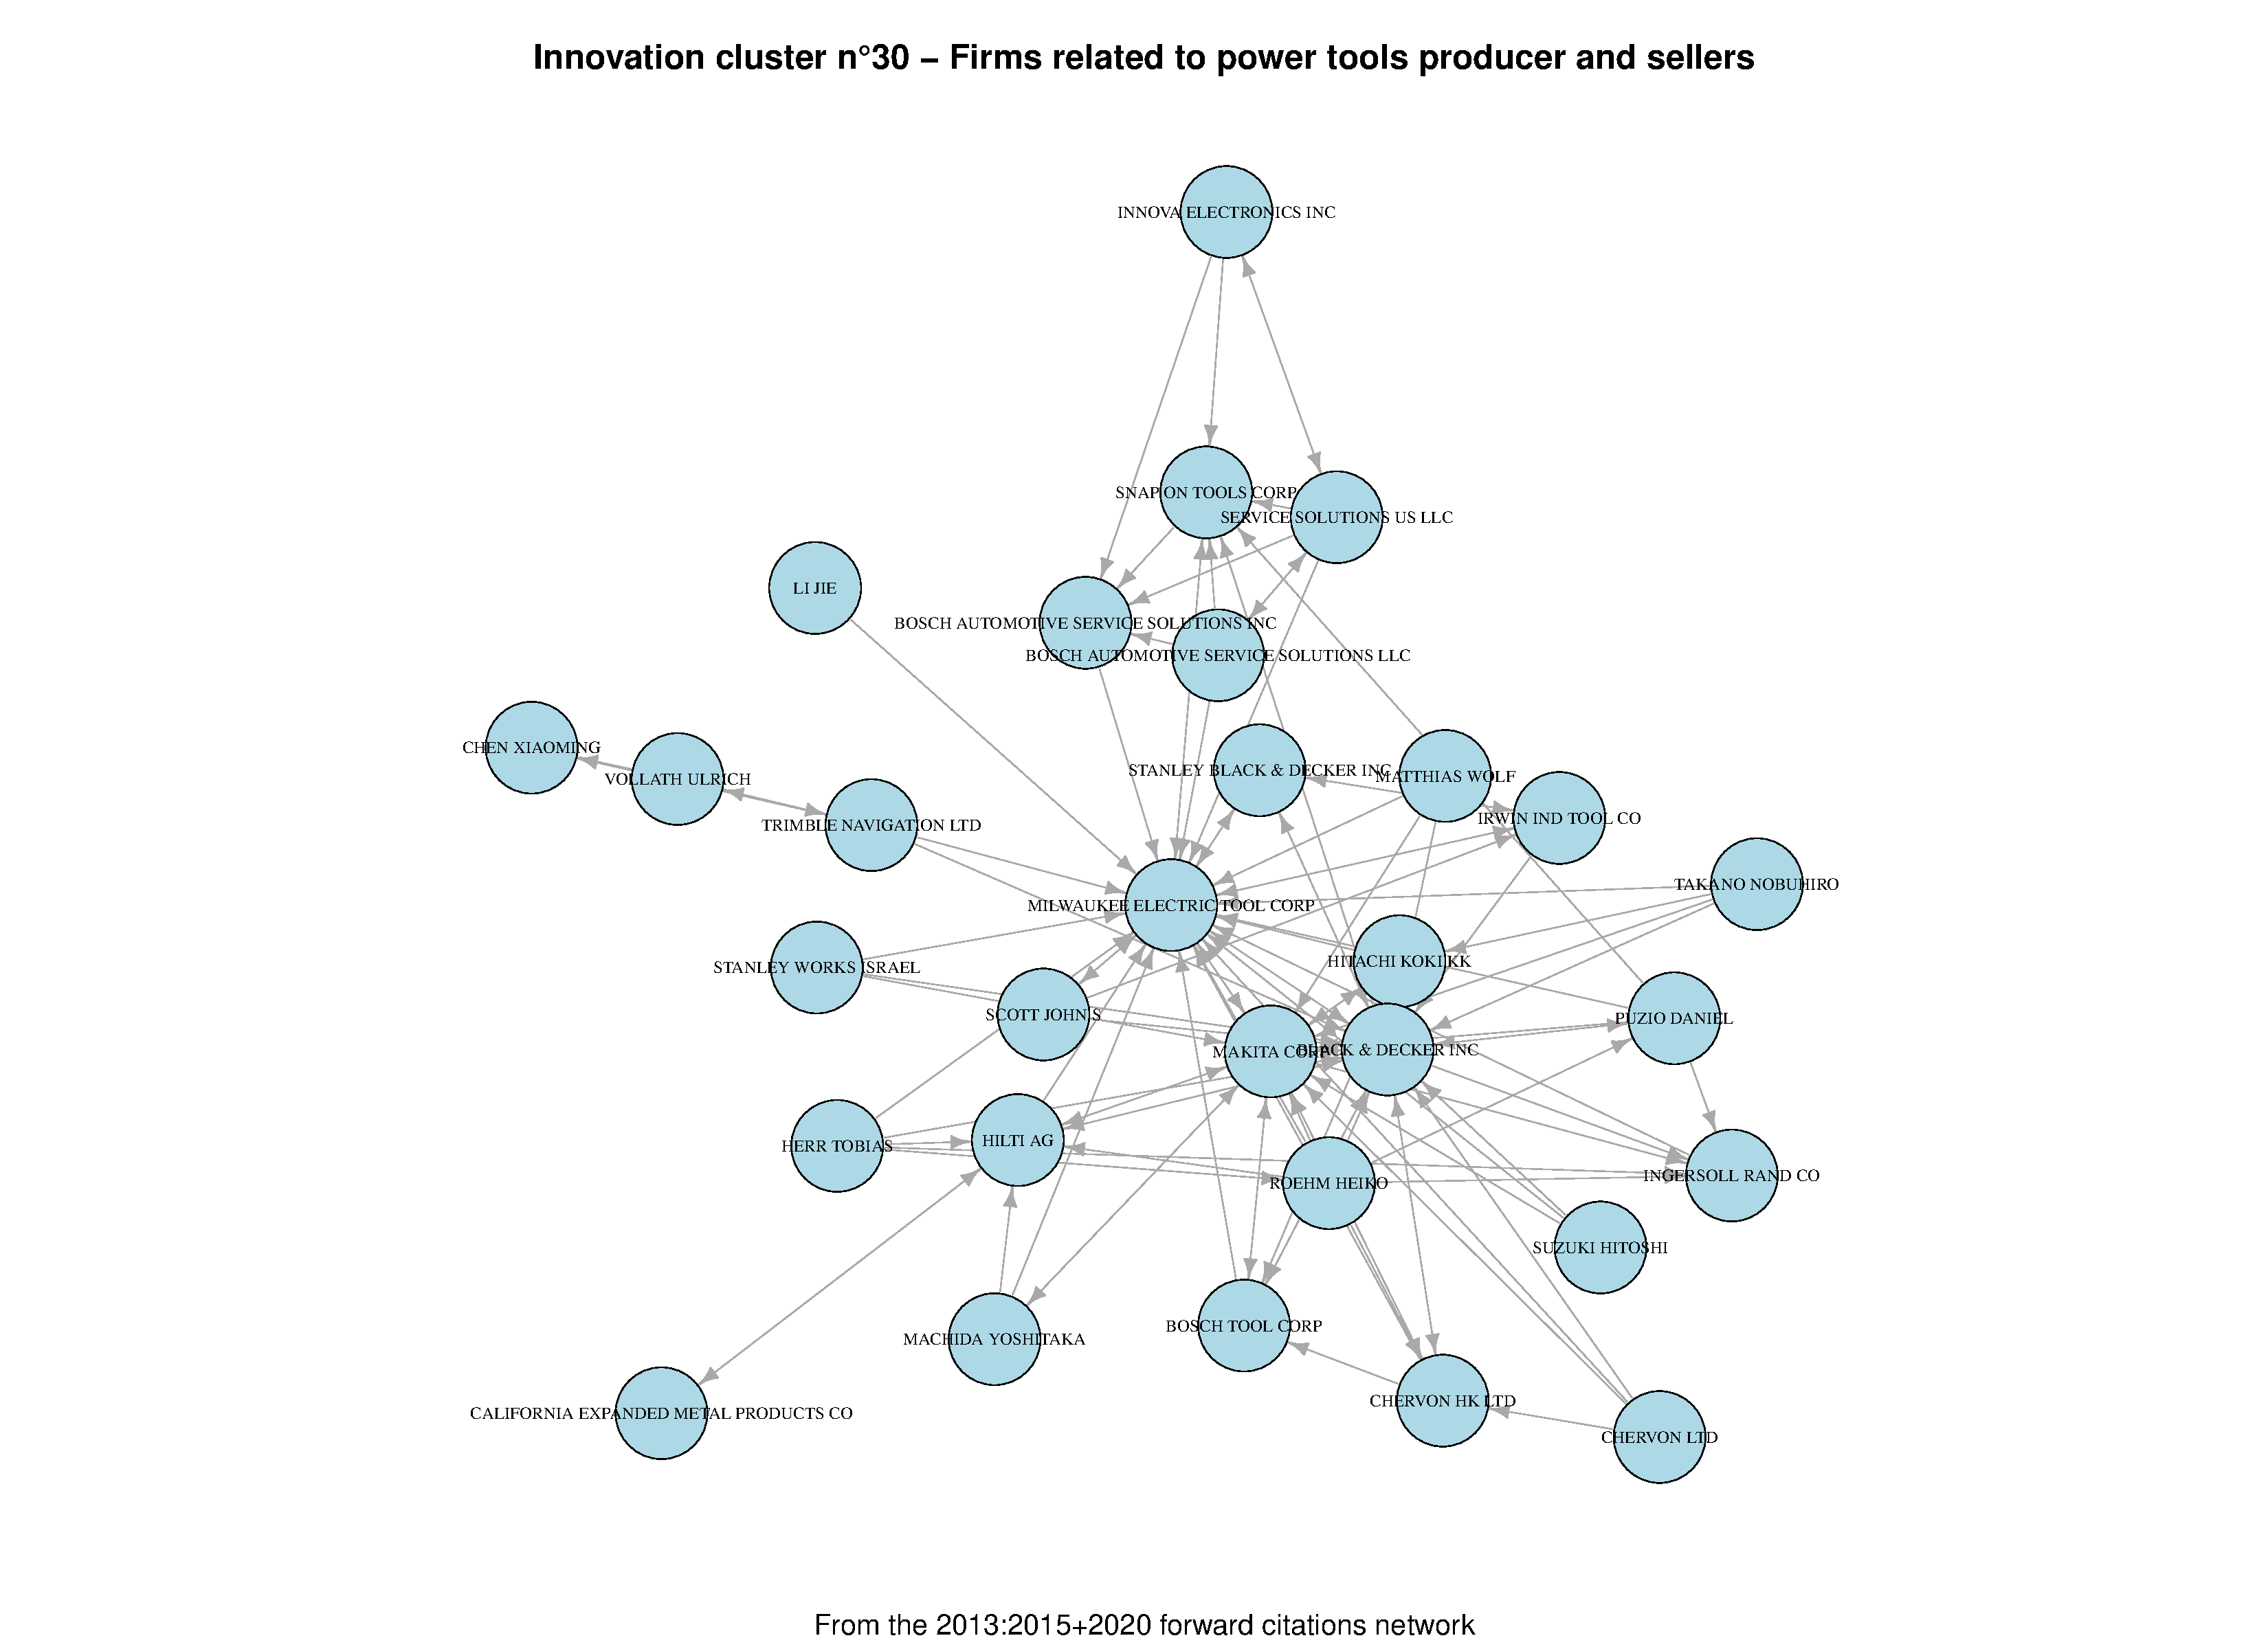
\includepdf[pages={1}]{clustering_example.pdf}

\end{document}